\begin{ceatitleframe}
     \maketitle
\end{ceatitleframe}



\begin{frame}{Binary code analysis: Why?}
       \placetextbox{0.25}{0.8}{\tiny \mybluebox{
        \begin{tabular}{l} 
          Source program \\
          \hline
          Ada\\
          C/C++\\
          Java\\ 
          Perl\\
          Python\\
          ...
        \end{tabular}}
       }
       
       \placetextbox{0.5}{0.7}{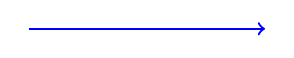
\begin{tikzpicture}
       \draw[->,blue,thick] (15,1) -- (18,1);
       \end{tikzpicture}}

       \placetextbox{0.5}{0.8}{\tiny \mybluebox{
       \begin{tabular}{l}
       Compiler 
       \end{tabular}}}

       \placetextbox{0.8}{0.8}{\tiny \mybluebox{
       \begin{tabular}{l} 
       Binary program\\
       \hline
       001011010101100\\
       100010101101010\\
       0101101010101101\\
       001011010101100\\
       100010101101010\\
       ...
       \end{tabular}}}


       \only<2->{\placetextbox{0.25}{0.5}{\scriptsize \mybox{
       \begin{tabular}{l}
       Static analysis
       \end{tabular}}}}

       \only<3->{\placetextbox{0.5}{0.5}{\scriptsize \mybox{
       \begin{tabular}{l}
       Certified compiler
       \end{tabular}}}}

       \only<4->{\placetextbox{0.8}{0.5}{\scriptsize \mygreenbox{
       \begin{tabular}{l}
       Static analysis
       \end{tabular}}}}

       \only<4->{\placetextbox{0.65}{0.35}{\scriptsize \mygreenbox{
       \begin{tabular}{l}
       $\bullet$ Alternative to source code analysis\\
       \hspace{0.4cm} $\bullet$ Compiler independent!\\
       \hspace{0.4cm} $\bullet$ Multi-languages programs
       \medskip \\
       $\bullet$ Analysis without access to source code\\
       \hspace{0.4cm} $\bullet$ Proprietary software \\
       \hspace{0.4cm} $\bullet$ Analysis of malware
       \end{tabular}}}}
\end{frame}



\begin{frame}{Challenges of binary code analysis}
  \begin{itemize}
  \item Low-level semantics of data
   \begin{itemize}
   \item Machine arithmetic, bit-level operations
   \item Systematic usage of untyped memory [big array]
   \item[] {\color{red}{Difficult for current formal techniques}}
   \end{itemize}
   \bigskip
   \item Low-level semantics of control
   \begin{itemize}
   \item No clear distinction data / instructions
   \item Dynamic jumps ({\tt jump eax})
   \item[] {\color{red}{No easy syntactic recovery of CFG}}
   \end{itemize}
   \bigskip
   \item Diversity of architectures and instruction sets 
   \begin{itemize}
   \item Too many instructions (ex. X86, $\geq900$ instructions)
   \item Modeling issues: side effect, addressing modes, prefixes, ...
   \end{itemize}
   \end{itemize}
\end{frame}



\begin{frame}{State of the art}
\begin{center}
\ovalbox{Nice progress since 2005}
\end{center}
\begin{itemize}
\item Intermediate languages:\\ {\color{red}{DBA}}~\citat{CEA}, BIL~\citat{CMU}, REIL~\citat{Zynamics}, ...
\medskip
\item Control flow reconstruction
\begin{itemize}
\item Unsafe static disassembly (linear sweep, recursive traversal)
\item Dynamic approach (under-approximation of actual CFG)
\item Safe static approach \\
{\color{red}{CFGBuilder}}~\citat{CEA}, Jakstab~\citat{TU München}, CodeSurfer/x86~\citat{GrammaTech}
\end{itemize}
\medskip
\item Test generation
\begin{itemize}
\item {\color{red}{OSMOSE}}~\citat{CEA}, SAGE~\citat{Microsoft}, Mayhem~\citat{ForAllSecure}
\end{itemize}
%\item Major relative works
%\item My position relative to them
\end{itemize}
\end{frame}


%% \begin{frame}{Binary code analysis: Challenges}
%%      \begin{center}
%%      \begin{tikzpicture}
%%      \begin{axis}[axis lines=none,ybar, ymin=0, width=10cm, height=7cm, enlarge y limits=0.5,
%%      ylabel={NB instructions},
%%      symbolic x coords={PPC, X86, DBA, Extended DBA},
%%      xtick=data,
%%      nodes near coords, nodes near coords align={vertical},
%%      ]
%%      \addplot coordinates {(PPC,1000) (X86,900) (DBA,4) (Extended DBA, 12)};
%%      \end{axis}
%%      \end{tikzpicture}%
%%      \end{center}

%%      \placetextbox{0.23}{0.7}{\scriptsize \mywhitebox{\color{blue}{+ 1000}}}

%%      \placetextbox{0.42}{0.67}{\scriptsize \mywhitebox{\color{blue}{+ 900}}}

%%      \placetextbox{0.23}{0.3}{\scriptsize \mywhitebox{\color{blue}{PPC}}}

%%      \placetextbox{0.42}{0.3}{\scriptsize \mywhitebox{\color{blue}{X86}}}

%%      \placetextbox{0.6}{0.3}{\scriptsize \mywhitebox{\color{blue}{DBA}}}

%%      \placetextbox{0.78}{0.3}{\scriptsize \mywhitebox{\color{blue}{DBA ++}}}

%%      \only<2->{\placetextbox{0.33}{0.62}{\scriptsize \myredbox{
%%      \begin{tabular}{l} 
%%      $\bullet$ Code and data ambiguity\\
%%      $\bullet$ No fixed procedure layout \\
%%      $\bullet$ No symbol information\\
%%      $\bullet$ Low-level semantics\\
%%      $\bullet$ Too many instructions\\
%%      $\bullet$ Indirect branches\\
%%      $\bullet$ Pervasive side-effect
%%      \end{tabular}}}}

%%      \only<3->{\placetextbox{0.7}{0.62}{\scriptsize \mygreenbox{
%%      \begin{tabular}{l} 
%%      $\bullet$ Simple, concise formalism
%%      \end{tabular}}}}

%% \end{frame}









%% \begin{frame}{Challenges}
%%      \begin{itemize}

%%      \item Binary code analysis
%%      \begin{itemize}
%%      \item Low-level data semantics
%%      \item Low-level control semantics
%%      \item Complex instruction sets
%%      \end{itemize}

%%      \medskip

%%      \item Large public software
%%      \begin{itemize}
%%      \item Dynamic memory allocation
%%      \item External libraries
%%      \item Compiled C/C++ program
%%      \end{itemize}


%%      \bigskip


%%      \item {\scriptsize Other challenges \color{red}{(out of scope)}:}
%%      \begin{itemize}
%%      \item {\scriptsize Self-modification}
%%      \item {\scriptsize Obfuscation}
%%      \item {\scriptsize Anti-desassembly protection}
%%      \item {\scriptsize Multithreading/ floats}
%%      \end{itemize}

%%      \end{itemize}
%% \end{frame}





\begin{frame}{Objectives}
     \begin{itemize}
     \item[\textbf{Goal}:] From embedded software to "grand public" software
     \begin{itemize}
     \item dynamic memory allocation
     \item large program size
     \item libraries
     \end{itemize}
     \end{itemize}
     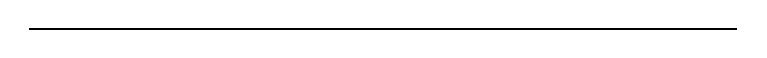
\begin{tikzpicture}
     \draw [thick, -] (1,1) -- (10,1);
     \end{tikzpicture}
     \begin{itemize}
     \item Generic formal model support
     \begin{itemize}
     \item More abstraction and specification
     \item Allow scalable analyses
     \end{itemize}
     \medskip
     \item Core Services for binary analysis
     \begin{itemize}
     \item X86 support
     \item Formal stubs for external libraries
     \end{itemize}
     \end{itemize}
\end{frame}




\begin{frame}{Achievements}
      \begin{itemize}
      \item \textbf{Semantics}~\citat{paper in progress}
      \begin{itemize}
      \item Extended DBA model
      \item New low-level region-based memory model
      \end{itemize}
      \bigskip
      \item \textbf{Platform: disassembly, simulation, analysis}~\citat{TACAS 2015}
      \begin{itemize}
      \item X86 decoding, disassembly algorithms, Formal stubs
      \item Simulation with different semantics
      \item Static analysis interface with fixpoint computation
      \end{itemize}
      \end{itemize}
\end{frame}



\section{Introduction}
\section{Low level semantics}

\subsection{Extended DBA}

\begin{frame}{DBA [Bardin et al, 2011]}
     \begin{columns}
     \begin{column}{0.5\linewidth}
     \tiny
     \vspace{-1cm}
     \begin{itemize}
     \item[] {\Huge \bf {\color{blue}4}} {\Large Instructions}
     \vspace{4cm}
     \item[] {\Huge \bf {\color{blue}29}} {\Large Operators}
     \end{itemize}
     \end{column}
     \tiny
     \begin{column}{0.5\linewidth}
     \begin{itemize}
     \item[] \tt lhs := e;
     \item[] \tt goto e; $<call, return>$
     \item[] \tt goto bv; $<call, return>$
     \item[] \tt ite (e)? goto $bv$ : goto $bv$
     \vspace{3cm}
     \item[] \tt v , {\color{red}{bv}}
     \item[] \tt @(e, $\leftarrow$, {\color{blue}{$k$}}), @(e, $\rightarrow$, {\color{blue}{$k$}})
     \item[] \tt e $\lbrace$ {\color{blue}{i}}.. {\color{blue}{j}}$\rbrace$, {\color{green!50!red}{$ext_{u,s}$}}(e, {\color{blue}{$n$}})
     \item[] \tt e $\lbrace$ {\color{green!50!red}{$+$, $-$, $\times$, $/_{u,s}$, $\%_{u,s}$}} $\rbrace$ e  
     \item[] \tt e $\lbrace$ {\color{green!50!red}{$\wedge, \vee, \oplus$, $>>$, $<<_{u, s}$, $::$}} $\rbrace$ e
     \item[] \tt e $\lbrace$ {\color{green!50!red}{$<_{u,s}$, $\leq_{u,s}$, $=$, $\neq$, $\geq_{u, s}$, $>_{u,s}$}} $\rbrace$ e
     \end{itemize}
     \end{column}
     \end{columns}
     {\begin{textblock*}{60mm}(8mm,0.42\textheight)
     \begin{blueblock}{Principles}
     \scriptsize
     \begin{itemize}
     \item[$\bullet$] Memory = Array of bytes
     \item[$\bullet$] Value = Bit-vector (01010110101...)
     \item[$\bullet$] Expression size statically known
     \item[$\bullet$] 1 machine instruction = 1 DBA block
     \item[$\bullet$] Standard operations on bit-vectors
     \end{itemize}
     \end{blueblock}
     \end{textblock*}}
     \only<2->{\begin{textblock*}{50mm}(72mm,0.42\textheight)
     \begin{greenblock}{Advantages}
     \scriptsize
     \begin{itemize}
     \item[$\bullet$] Platform-independent
     \item[$\bullet$] Concise set of instructions
     \item[$\bullet$] Free of side-effect
     \item[$\bullet$] Bit precise modeling
     \end{itemize}
     \end{greenblock}
     \end{textblock*}}
     \only<3->{\begin{textblock*}{50mm}(72mm,0.42\textheight)
     \begin{redblock}{Issues}
     \scriptsize
     \begin{itemize}
     \item[$\bullet$] No specification
     \item[$\bullet$] No abstraction (memory alloc)
     \item[$\circ$] No self-modification
     \item[$\circ$] No floats, threads, interrupts ...
     \end{itemize}
     \end{redblock}
     \end{textblock*}}
\end{frame}


\begin{frame}{DBA ++}
     \begin{columns}
     \begin{column}{0.5\linewidth}
     \tiny
     \vspace{-1cm}
     \begin{itemize}
     \item[] {\Huge \bf {\color{blue}11}} {\Large Instructions}
     \vspace{4cm}
     \item[] {\Huge \bf {\color{blue}29}} {\Large Operators}
     \end{itemize}
     \end{column}
     \tiny
     \begin{column}{0.5\linewidth}
     \begin{itemize}
     \item[] \tt lhs := e;
     \item[] \tt goto e; $<call, return>$
     \item[] \tt goto bv; $<call, return>$
     \item[] \tt ite (e)? goto $bv$ : goto $bv$
     \item[] \tt {\color{blue}{stop $<ok, ko, unsupported, bad>$};}
     \item[] \tt {\color{blue}{lhs := nondet (?region)}; }
     \item[] \tt {\color{blue}{lhs := undef}; }
     \item[] \tt {\color{blue}{assert (cond)}; }
     \item[] \tt {\color{blue}{assume (cond)};}
     \item[] \tt {\color{blue}{lhs := malloc (size)}; }
     \item[] \tt {\color{blue}{free (expr)};}
     \bigskip
     \item[] \tt v $<flag, temp>$, {\color{red}{(r, bv), $\bot_V$}}
     \item[] \tt @(e, $\leftarrow$, $k$), @(e, $\rightarrow$, $k$)
     \item[] \tt e $\lbrace$ i.. j$\rbrace$, $ext_{u,s}$(e, $n$)
     \item[] \tt e $\lbrace$ $+$, $-$, $\times$, $/_{u,s}$, $\%_{u,s}$ $\rbrace$ e  
     \item[] \tt e $\lbrace$ $\wedge, \vee, \oplus$, $>>$, $<<_{u, s}$, $::$ $\rbrace$ e
     \item[] \tt e $\lbrace$ $<_{u,s}$, $\leq_{u,s}$, $=$, $\neq$, $\geq_{u, s}$, $>_{u,s}$ $\rbrace$ e
     \end{itemize}
     \end{column}
     \end{columns}
     \begin{textblock*}{60mm}(8mm,0.45\textheight)
     \begin{blueblock}{Principles}
     \scriptsize
     \begin{itemize}
     \item[$\bullet$] Memory = Distinct regions of bytes 
     \item[$\bullet$] High-level operations
     \item[$\bullet$] Access permissions {\tiny (R/W/X $\rightarrow$ region $\rightarrow \phi$)}
     \end{itemize}
     \end{blueblock}
     \end{textblock*}
\end{frame}


\begin{frame}{Extended DBA model}
     \textbf{Former DBAs limitations}~\citat{Bardin et al, 2011}:
     \begin{itemize}
     \item Flat memory model
     \item Losing precision on a write affects {\color{red}{all memory space}} 
     \end{itemize}
     \medskip
     \textbf{Extended DBAs}~\citat{Djoudi \& Bardin, 2013}:
     \begin{itemize}
     \item Region-based memory model (Compcert like)
     \item Losing precision on a write affects {\color{blue}{a single memory region}}  
     \end{itemize}
     \bigskip
     \begin{columns}[t]
     \begin{column}[T]{3.7cm}
     \underline{\it{Basic values}:}
     \begin{itemize}
     \item (region, bitvector)
     \item ${\color{red}{\bot_V}}$
     \end{itemize}
     \end{column}
     \pause
     \begin{column}[T]{6cm}
     \underline{\it{Problem}:}
     \begin{itemize}
     \item Most of operations are illegal: $({\color{red}{r_1}}, v_1) + ({\color{red}{r_2}}, v_2)$ = ${\color{red}{\bot_V}}$
     \end{itemize}
     \end{column}
     \end{columns}
\end{frame}



\begin{frame}[fragile]{Memcopy}
     \lstset{basicstyle=\tiny, stepnumber=10000, language=C}
     \begin{lstlisting} 
     void* memcpy (void* dest , const void* src , unsigned int n) 
      { unsigned int i; 
        for (i = 0; i < n ; i++)
          ((char*) dest) [i] = ((const char*) src) [i]; 
        return dest;
      }

     int** main ( ) 
      {
        int a = 1, b = 2, c = 3;
        const int* e [3] = {&a ,&b ,&c};
        int* d [3] = {(int*) 0, (int*) 0, (int*) 0} ; //NULL
        memcpy (d, e, 3 * sizeof (int));
        return d ;
      }
     \end{lstlisting}
     \only<2>{\placetextbox{0.75}{0.68}{\scriptsize \mybox{\begin{tabular}{l} $\bullet$ Deconstruction/Reconstruction of pointers \\ $\bullet$ Not representable with standard regions
%% @(Stack, dest) = & (Stack, \&a)\{0, 7\}\\ @(Stack, dest+1) = & (Stack, \&a)\{8, 15\}\\ @(Stack, dest+2) = &(Stack, \&a)\{16, 23\}\\ ...
     \end{tabular}}}}
\end{frame}


\begin{frame}[fragile]{Memmove}
      \lstset{basicstyle=\tiny, stepnumber=10000, language=C}
      \begin{lstlisting}
      void* memmove (void *dest, const void *src, unsigned int n)
       {
          unsigned int i;
          unsigned char *pd = dest;
          const unsigned char *ps = src;
          €{\color{red}{if (ps $<$ pd)}}€
              for (i = n - 1; i >= 0 ; i--) pd [i] = ps [i]; 
          €{\color{red}{else}}€
              for (i = 0; i < n ; i++) pd [i] = ps [i]; 
          return dest;
       }

      int main(){
        int j;
        int* res;
          int a = 1, b=2, c=3;
          int* src[3] = {&a,&b,&c};
          int* dest = (int *) malloc (3 * sizeof (int*));
          memmove(dest,src,3*sizeof(int*));
          res = dest;
        return *res;
      }
      \end{lstlisting}
      \only<2>{\placetextbox{0.75}{0.68}{\mybox{\scriptsize\begin{tabular}{l} $\bullet$ Comparison between pointers \\ $\bullet$ Not representatble with standard regions
      %% \only<2>{\placetextbox{0.75}{0.68}{\tiny \mybox{\begin{tabular}{ll} if  (Stack, ps) $<$ (Malloc1, pd)  & \\ @(Malloc1, pd + n - 1) = & (Stack, \&c)\{24, 31\}\\ @(Malloc1, pd + n - 2) = & (Stack, \&c)\{16, 23\}\\ @(Malloc1, pd + n - 3) = &(Stack, \&c)\{8, 15\}\\ ... & \\ else & \\ @(Malloc1, pd) = & (Stack, \&a)\{0, 7\}\\ @(Malloc1, pd + 1) = & (Stack, \&a)\{8, 15\}\\ @(Malloc1, pd + 2) = &(Stack, \&a)\{16, 23\}\\ ...
      \end{tabular}}}}
\end{frame}


\begin{frame}{Low-level region-based memory model (1)}
    \begin{columns}[t]
     \begin{column}[T]{3.7cm}
      \textbf{New values:}
      \begin{scriptsize}
      \begin{itemize}
      \item (region, bitvector)
      \item \textbf{\color{blue}{Symbol}}
      \item $\bot_V$
      \end{itemize}
      \end{scriptsize}   
     \end{column}
     \pause
     \begin{column}[T]{6cm}
      \textbf{Principles:}
      \begin{tiny}
      \begin{itemize}
      \item Ideally no illegal operations
      \item Propagation of symbolic values
      \item Error on (\texttt{\color{red}{load, store, jump, ite}})
      \item Need to $simplify:$ $Symbol \rightarrow \lbrace {\color{blue}{Value(region, bv)}} \rbrace$    
      \end{itemize}
      \end{tiny}
     \end{column}
     \end{columns}
     \pause
     \bigskip
      \textbf{Example1}:  ($Stack$, 5)\{16,32\} $::$ ($Stack$, 5)\{0,15\}

      \medskip

      \textbf {Without symbolic values}
      \begin{itemize}
      \item ($Stack$, 5)\{16,32\} $::$ ($Stack$, 5)\{0,15\} = {\color{red}{$\bot_V$}} $::$ {\color{red}{$\bot_V$}} = {\color{red}{$\bot_V$}}
      \end{itemize}
      \pause
      \medskip

      \textbf{With symbolic values}
      \begin{itemize}
      \item ($Stack$, 5)\{16,32\} $::$ ($Stack$, 5)\{0,15\}  = \\ {\color{blue}{Restrict(($Stack$, 5), 16,32)}} $::$ {\color{blue}{Restrict(($Stack$, 5),0,15)}} = \\ {\color{red}{($Stack$, 5)}}
      \end{itemize}
\end{frame}


\begin{frame}{Low-level region-based memory model (2)}
      \begin{columns}[t]
     \begin{column}[T]{3.7cm}
      \textbf{New values:}
      \begin{scriptsize}
      \begin{itemize}
      \item (region, bitvector)
      \item \textbf{\color{blue}{Symbol}}
      \item $\bot_V$
      \end{itemize}
      \end{scriptsize}   
     \end{column}
     \begin{column}[T]{6cm}
      \textbf{Principles:}
      \begin{tiny}
      \begin{itemize}
      \item No illegal operations
      \item Propagation of symbolic values
      \item Error on (\texttt{\color{red}{load, store, jump, ite}})
      \item Need to $simplify:$ $Symbol \rightarrow \lbrace {\color{blue}{Value(region, bv)}} \rbrace$    
      \end{itemize}
      \end{tiny}
     \end{column}
     \end{columns}

      \bigskip
      \textbf{Example2}: $($Stack$, 5) + ($Stack$, 6) - ($Stack$, 4)$

      \medskip


      \textbf{Without symbolic values}
      \begin{itemize}
      \item (Stack$, 5) + ($Stack$, 6) =$ {\color{red}{$\bot_V$}}
      \item $\bot_V \ -$ (Stack, $4) =$ {\color{red}{$\bot_V$}} 
      \end{itemize}
      \pause

      \medskip

      \textbf{With symbolic values}
      \begin{itemize}
      \item (Stack$, 5) +$ (Stack, 6) = {\color{blue}{$\sum$(2 $\times$ Stack,11)}} 
      \item  {$\sum$(2 $\times$ Stack,11)} - (Stack, 4) = {$\sum$(1 $\times$ Stack,7)} 
      \item {$\sum$(1 $\times$ Stack,7)} =  {\color{red}{(Stack,7)}}
      \end{itemize}
\end{frame}



\begin{frame}{Low-level region-based memory model (3)}
\begin{columns}[t]
     \begin{column}[T]{3.7cm}
      \textbf{New values:}
      \begin{scriptsize}
      \begin{itemize}
      \item (region, bitvector)
      \item \textbf{\color{blue}{Symbol}}
      \item $\bot_V$
      \end{itemize}
      \end{scriptsize}   
     \end{column}
     \begin{column}[T]{6cm}
      \textbf{Principles:}
      \begin{tiny}
      \begin{itemize}
      \item No illegal operations
      \item Propagation of symbolic values
      \item Error on (\texttt{\color{red}{load, store, jump, ite}})
      \item Need to $simplify:$ $Symbol \rightarrow \lbrace {\color{blue}{Value(region, bv)}} \rbrace$    
      \end{itemize}
      \end{tiny}
     \end{column}
     \end{columns}
      \bigskip
      \begin{center}
      \begin{tabular}{|l|c|c|}
      \hline 
       model     & simulation &  scalability of analysis  \\ %&  détection  &  exploitabilité   \\
       %           &           &   analysis        \\ %    &  de bugs    &     \\
      \hline
      flat        & \mycheckmark  & \mybadmark  \\ % & \mybadmark & \mybadmark  \\
      \hline
      region      & \mybadmark & \mycheckmark  \\ % & \mycheckmark  & \mybadmark  \\
      \hline
      \textbf{low-level region}      & \mycheckmark & \mycheckmark  \\ % & \mycheckmark  & ??  \\
      \hline
      \end{tabular}
      \end{center}

      %% \begin{scriptsize}
      %% \begin{itemize}
      %% \item Order of evaluation of operands may be important
      %% \item Rewriting rules on symbolic values (try to recover concrete values)
      %% \end{itemize}
      %% \end{scriptsize}
      %% \textbf{Examples}
      %% \begin{center}
      %% \begin{tabular}{|c|c|c|}
      %% \hline
      %%  & regions & low-level regions\\
      %% \hline
      %% {\scriptsize $(Stack, 5) + (Stack, 6) - (Stack, 4)$} & $\bot$ & {\scriptsize $(Stack, 7)$}\\
      %% \hline
      %% Write $(Stack, 5)$  & $\bot$, $\bot$ & {\scriptsize $(Stack, 5)_{\color{red}{\{0, 7\}}}$, $(Stack, 5)_{\color{blue}{\{7, 15\}}}$}\\
      %% \hline
      %% Read ({\scriptsize $(Stack, 5)_{\color{red}{\{0, 7\}}}$, $(Stack, 5)_{\color{blue}{\{7, 15\}}}$}) & - & $(Stack, 5)$\\
      %% \hline
      %% \end{tabular}
      %% \end{center}
\end{frame}



\subsection{Four semantics modes}


%% \begin{frame}{Symbolic evaluation issues}
%%        \begin{itemize}
%%        \item $Symbol$ causes error on (\texttt{\color{red}{load, store, jump, ite}})
%%        \end{itemize}
%%        \bigskip
%%        \begin{itemize}
%%        \item Lazy simplification of symbolic values
%%        \medskip
%%        \begin{itemize}
%%        \item $simplify:$ $Symbol \rightarrow \lbrace {\color{blue}{Value(region, bv)}}, {\color{orange}{NoSimp_\top}}, {\color{red}{NoSimp_\bot}} \rbrace$
%%        \medskip
%%        \begin{itemize}
%%        \item \begin{scriptsize}
%%        {\color{blue}{$Value(region, bv)$}}: Simplification returns a value (r, bv)\\
%%        eg.~$Expr(2\times(Stack, 2) - (Stack, 0)) = (Stack, 4)$  
%%        \end{scriptsize}
%%        \bigskip
%%        \item \begin{scriptsize}
%%        {\color{orange}{$NoSimp_\top$}} : No simplification, future simplification maybe possible \\
%%        eg.~$Expr(2\times(Stack, 2))$
%%        \end{scriptsize}
%%        \bigskip
%%        \item \begin{scriptsize}
%%        {\color{red}{$NoSimp_\bot$}} : No simplification, future simplification impossible\\
%%        eg.~typically, unsatisfiable constraints on regions %%$Expr((Stack, 5) > (Stack, 12))$
%%        \end{scriptsize}
%%        \end{itemize}
%%        \end{itemize}
%%        \end{itemize}
%% \end{frame}



\begin{frame}{Simplification algorithm}
        \begin{itemize}
        \item basicSymbol: Rewriting rules (Efficient)~\citat{A. Djoudi}
        \begin{itemize}
        \item basicSymbol :=\\
        \begin{scriptsize}
        \hspace*{1cm}$\mid$ Symb (region, bitvector)\\
        \hspace*{1cm}$\mid$ Restrict (symbol,$ o_1, o_2$), $o_1, o_2 \in \mathbb{N}$\\
        \hspace*{1cm}$\mid$ $\sum (c_i .$ symbol) with $c_i \in \mathbb{N}$\\
        \end{scriptsize}
        \item Sound \& efficient rewriting rules
        \item Incomplete
        \end{itemize}
        \bigskip
        \item logicSymbol: Logical encoding (Complete)~\citat{P. Wilke}
        \begin{itemize}
        \item No term restriction
        \item Encoding the problem into two BV-SAT problems
        \begin{itemize}
        \item $1^{st}$ solving: get one possible simplification
        \item $2^{nd}$ solving: check uniqueness
        \end{itemize}
        \item Expensive
        \end{itemize}
        \end{itemize}
\end{frame}


%% \begin{frame}{Simplification of symbolic values}
      %% \begin{itemize}
      %% \item Need to simplify symbolic values at some instructions (ite, goto, ...) to avoid errors
      %% \bigskip
      %% \item $simplify:$ $Symbol \rightarrow \lbrace Value(region, bv), NoSimp_\top, NoSimp_\bot \rbrace$
      %% \begin{itemize}
      %% \item \begin{scriptsize}
      %% $Value(r, bv)$: Simplification return a value (r, bv)\\
      %% eg.~$Expr(2\times(Stack, 2) - (Stack, 0)) = (Stack, 4)$  
      %% \end{scriptsize}
      %% \bigskip
      %% \item \begin{scriptsize}
      %% $NoSimp_\top :$ No simplification, future simplification maybe possible \\
      %% eg.~$Expr(2\times(Stack, 2))$
      %% \end{scriptsize}
      %% \bigskip
      %% \item \begin{scriptsize}
      %% $NoSimp_\bot :$ No simplification, future simplification impossible\\
      %% eg.~typically, unsatisfiable constraints on regions %%$Expr((Stack, 5) > (Stack, 12))$
      %% \end{scriptsize}
      %% \end{itemize}
      %% \medskip
      %% \item Use: Simplification after each $eval$
      %% \end{itemize}
%% \end{frame}


%% \begin{frame}{Simplification points}
      %% \begin{itemize}
      %% \item Where to simplify?
      %% \begin{itemize}
      %% \item Query points (ite, goto x, $@[x] := ..$) // error cases
      %% \item Propagation points 
      %% \end{itemize}
      %% \bigskip
      %% \item In query pts: (simplification is mandatory)
      %% \begin{itemize}
      %% \item $simplify(symb) = Value(r,bv)$ $\Rightarrow$ recovered value
      %% \item $simplify(symb) = NoSimp_\top$ $\Rightarrow$ $Undef$ (cannot propagate)
      %% \item $simplify(symb) = NoSimp_\bot$ $\Rightarrow$ $Undef$ (cannot propagate)
      %% \end{itemize}
      %% \bigskip
      %% \item In propagation pts : (simplification is optional)
      %% \begin{itemize}
      %% \item $simplify(symb) = Value(r, bv)$ $\Rightarrow$ recovered value
      %% \item $simplify(symb) = NoSimp_\top$ $\Rightarrow$ keep $symb$ and delay simplification      
      %% \item $simplify(symb) = NoSimp_\bot$ $\Rightarrow$ $Undef$ (hopeless to propagate $symb$)
      %% \end{itemize}
      %% \end{itemize}
%% \end{frame}



\begin{frame}{Simplification process [Wilke-Besson]}
      \begin{small}
      $$
      \begin{cases}
      \symb : &$ terms built from $ r \in \mathcal{R} \\
      \varsymb : &$ terms built from $ X_r $ variables s.t. $ \varsymb = \symb[X_r/r]\\
      Symb^\# & = \{\varsymb, \symb \in \fullsymb\}\\
      \end{cases}
      $$
      \end{small}
      \medskip
      Checking the following assertion using SMT-solvers~\citat{Wilke} :\\
      \begin{center}
      $\memmodel_\symb \wedge (\varsymb = (X_r + X_{bv})) \wedge \resconstraint_\symb $
      \end{center}
      \begin{itemize}
      \item $\memmodel_\symb:$ memory model constraints built from $\symb$
      %% \item $\condenv : $ condition environment
      \item $\tau_\symb : $ constraints on the result $(X_r, X_{bv})$ built from $\symb$
      \item $\varsymb = (X_r + X_{bv}): $ in order to simplify $\symb$ as a $Value(r,bv)$
      \end{itemize}
      %% \placetextbox{0.84}{0.5}{\tiny \myredbox{
      %% \begin{tabular}{l} 
      %% Step 1: get one possible solution\\
      %% Step 2: check uniqueness
      %% \end{tabular}}}

\end{frame}


\begin{frame}{Memory model constraints [Wilke-Besson]}
      $\symb \in \fullsymb, \memmodel_\symb \in \varfullsymb$, $S_r: $ size of region $r$ \\
      \vspace{1cm}
      \begin{scriptsize}
      $$ 
      \memmodel_\symb = 
              \bigwedge \begin{dcases} 
                           X_{cst} = 0 \\ 
                           size(X_{stack}) < Max \wedge \bigwedge \limits_{r \in s, \atop {r \neq Stack, \atop r \neq Cst}} size(X_r) = S_r \qquad \qquad \qquad //\text{size constraints}\\ 
                           \bigwedge \limits_{r\neq cst \atop r \in \symb} ~ X_r \neq 0 \wedge X_r < X_r + size(X_r)  \qquad \qquad \qquad \qquad \qquad //\text{no overflow}\\
                           \bigwedge \limits_{(r,off) \in \symb \atop r\neq cst} 0 \leq off < size (X_r) \qquad \qquad \qquad \qquad \qquad \qquad \qquad //\text{legal access} \\
                           \bigwedge \limits_{r_1, r_2 \in \symb, \atop {r_1, r_2 \neq cst \atop r_1 \neq r_2}} (X_{r_1} > X_{r_2} + size(X_{r_2}) \vee X_{r_2} > X_{r_1} + size(X_{r_1})) \qquad //\text{no overlap}
                        \end{dcases}
      $$

      \end{scriptsize}
      \only<1->{\placetextbox{0.5}{0.75}{\tiny \mywhiteblackbox{
      \begin{tikzpicture}
      \draw [thick, |-|] (1,0.1) -- (10,0.1)
      node[pos=0,mynode,fill=black,label=\textcolor{black}{$cst=0$}]{}
      node[pos=0.15,mynode,fill=orange,text=orange,label=\textcolor{orange}{$malloc1=?$}]{}
      node[pos=0.35,mynode,fill=red,text=red,label=\textcolor{red}{$malloc2=?$}]{}
      node[pos=0.7,mynode,fill=blue,text=blue,label=\textcolor{blue}{$stack = ?$}]{};
      \fill [orange] (2.3,0.07) rectangle (3,0.13);
      \fill [red] (4.2,0.07) rectangle (4.6,0.13);
      \fill [blue] (7.3,0.07) rectangle (9.97,0.13);
      \end{tikzpicture}
      }}}
\end{frame}


\begin{frame}{Result constraints [Wilke-Besson]}
      $\symb \in \fullsymb, \tau_\symb \in \varfullsymb$ \\
      \medskip
      A solution $(r, bv)$ of simplifying symbolic expression $\symb$ must verify:
      \medskip
      \begin{itemize}
      \item Case 1: pointer solution
      \begin{scriptsize}
      $$
      \tau_\symb = \bigwedge \begin{dcases}
                        \color{red}{\Big(\bigvee \limits_{r' \in \symb} X_r = X_{r'}\Big)} \qquad //X_r \text{ must appear syntactically in } \varsymb \\
                        X_{bv} < size(X_r)  \qquad \qquad //\text{valid pointer}
                        \end{dcases}
      $$
      \end{scriptsize}
      \medskip
      \item Case 2: Constant solution
      \begin{scriptsize}
      $$
      \hspace{-5.2cm}\tau_\symb = \bigwedge \begin{dcases}
                        X_r = 0 \\
                        0 \leq X_{bv} < Max
                        \end{dcases}
      $$
      \end{scriptsize}
      \end{itemize}
\end{frame}


%% \begin{frame}{Simplification algorithm(1)}
     %% \begin{scriptsize}
     %% $simplifyAsPtr : Symbol \rightarrow \lbrace Value(r, bv), NoPtr_\top, NoPtr_\bot\rbrace$\\
     %% \qquad $Value(r, bv):$ unique solution value $(r, bv)$ \\
     %% \qquad $NoPtr_\top: $ Too many possible solutions \\
     %% \qquad $NoPtr_\bot: $ No possible solution\\
     %% \medskip
     %% $simplifyAsCst : Symbol \rightarrow \lbrace Value(Cst, bv), NoCst_\top, NoCst_\bot\rbrace$\\
     %% \qquad $Value(Cst, bv):$ unique solution value $(Cst, bv)$ \\
     %% \qquad $NoCst_\top: $ Too many possible solutions\\
     %% \qquad $NoCst_\bot: $ No possible solution\\
     %% \begin{center}
     %% \begin{tabular}{|l|l|l|}
     %% \hline
     %% $simplifyAsPtr(s)$ & $simpifyAsCst(s)$ & $simplify(s)$\\
     %% \hline
     %% \hline
     %% $(R, bv_1)$ & $(Cst, bv_2)$ & Impossible (*)\\
     %% \hline
     %% $(R, bv_1)$ & $NoCst_\top$ & {\color{red}{$(R, bv_1)$}} \\
     %% \hline
     %% $(R, bv_1)$ & $NoCst_\bot$ & Impossible \\
     %% \hline
     %% $NoPtr_\top$ & $(Cst, bv_2)$ & {\color{blue}{$(Cst, bv_2)$}} \\
     %% \hline
     %% $NoPtr_\top$ & $NoCst_\top$ & $\nosimpltop$ \\
     %% \hline
     %% $NoPtr_\top$ & $NoCst_\bot$ & Impossible \\
     %% \hline
     %% $NoPtr_\bot$ & $(Cst, bv_2)$ & {\color{blue}{$(Cst, bv_2)$}} \\
     %% \hline
     %% $NoPtr_\bot$ & $NoCst_\top$ & $\nosimpltop$ \\
     %% \hline
     %% $NoPtr_\bot$ & $NoCst_\bot$ & $\nosimplbot$ \\
     %% \hline
     %% \end{tabular}
     %% \end{center}
     %% \medskip 
     %% (*): No duality [to be confirmed]
     %% \end{scriptsize}

%% \end{frame}


\begin{frame}{Simplification algorithm for binaries}
      \begin{scriptsize}
      \fbox{
      \begin{minipage}{0.96\textwidth}
      \centering
      \begin{tikzpicture}[->,>=stealth', every node/.style={scale=0.67}]
        %text width=3cm,
       \node[state] (logicSymbol)
       {\begin{tabular}{l} 	
        {\color{red}{logicSymbol}}
       \end{tabular}
       };


       \node[state, above of=logicSymbol, node distance=4.3cm, xshift=3cm, anchor=center] (phi)
       {\begin{tabular}{l}
        \texttt{$\memmodel$: memory model constraints} \\
        \texttt{$R^*$: Region symbol with R as value in the model}
       \end{tabular}
       };

       \node[state, right of=logicSymbol, node distance=3.5cm, anchor=center] (model1)
       {\begin{tabular}{l}
        \texttt{resolve smt assertions:}\\
         $\memmodel \models ({\color{red}{logicSymbol}} =  {\color{red}{(r+ bv)}}) \wedge$ \\
         \hspace{0.8cm} ${\color{red}{r}} \neq CST$
       \end{tabular}
       };

      \node[state, right of=model1, yshift=3cm, node distance=4cm, anchor=center] (sat1)
       {
       \begin{tabular}{l}
        \texttt{resolve smt assertions:}\\
        $\memmodel \models ({\color{red}{logicSymbol}}   =  {\color{red}{(r+ bv)}}) \wedge$ \\
        \hspace{0.8cm} ${\color{red}{(r+ bv)}} \neq {\color{blue}{(R^*+ BV)}}$
       \end{tabular}
       };


       \node[state, right of=sat1, yshift=2cm, node distance=1cm, anchor=center] (concrete1)
       {
       \begin{tabular}{l}
       ${\color{blue}{Value(R^*, BV)}}$
       \end{tabular}
       };


       \node[state, right of=sat1, yshift=-3cm, node distance=4cm, anchor=center] (sat2)
       {\begin{tabular}{l}
         \texttt{resolve smt assertions:}\\
        $\memmodel \models ({\color{red}{logicSymbol}}   =  {\color{red}{(r+ bv)}}) \wedge$ \\
        \hspace{0.8cm} ${\color{red}{(r+bv)}} \neq {\color{blue}{(R+ BV)}}$
       \end{tabular}
       };

       \node[state, right of=model1, yshift=-3cm, node distance=4cm, anchor=center] (model2)
       {
       \begin{tabular}{l}
         \texttt{resolve smt assertions:}\\
        $\memmodel \models ({\color{red}{logicSymbol}}   =  {\color{red}{(r+ bv)}}) \wedge$ \\
        \hspace{0.8cm} ${\color{red}{r}} = CST$
       \end{tabular}
       };


       \node[state, right of=model2, yshift=-2cm, node distance=1cm, anchor=center] (undef1)
       {
       \begin{tabular}{l}
        No solution:\\
        $\nosimplbot$
       \end{tabular}
       };


       \node[state, right of=sat2, yshift=2cm, node distance=1cm, anchor=center] (concrete2)
       {
       \begin{tabular}{l}
        ${\color{blue}{Value(Cst,BV)}}$
       \end{tabular}
       };


       \node[state, right of=sat2, yshift=-2cm, node distance=1cm, anchor=center] (undef2)
       {
       \begin{tabular}{l}
        Several possible solutions:\\
        $\nosimpltop$
       \end{tabular}
       };

       \path 
       (logicSymbol) edge (model1)
       (model1) edge node[sloped, above]{sat} node[sloped, below]{\hspace{0.2cm}{\color{red}{(r, bv)}} = {\color{blue}{(R, BV)}}} (sat1)
       (model1) edge node[sloped, below]{unsat} (model2)
       (sat1) edge node[sloped, above]{sat} (sat2)
       (sat1) edge node[sloped, below]{unsat} (concrete1)
       (model2) edge node[sloped, below]{unsat} (undef1)
       (model2) edge node[sloped, above]{sat} node[sloped, below]{\hspace{0.2cm}{\color{red}{(r, bv)}} = {\color{blue}{(R, BV)}}} (sat2)
       (sat2) edge node[sloped, below]{sat} (undef2)
       (sat2) edge node[sloped, below]{unsat} (concrete2)
       ;

      \end{tikzpicture}
      \end{minipage}
      }
      \end{scriptsize}
      %% \only<2>{\placetextbox{0.45}{0.35}{\tiny \mywhiteblackbox{
      %% \begin{tikzpicture}
      %% \draw [thick, |-|] (1,0.1) -- (10,0.1)
      %% node[pos=0,mynode,fill=black,label=\textcolor{black}{$cst=0$}]{}
      %% node[pos=0.15,mynode,fill=orange,text=orange,label=\textcolor{orange}{$malloc1$}]{}
      %% node[pos=0.19,label={[xshift=0cm, yshift=-0.7cm]\textcolor{purple}{$\uparrow \atop Value(R, BV)$}}]{}
      %% node[pos=0.35,mynode,fill=red,text=red,label=\textcolor{red}{$malloc2$}]{}
      %% node[pos=0.7,mynode,fill=blue,text=blue,label=\textcolor{blue}{$stack$}]{};
      %% \fill [orange] (2.3,0.07) rectangle (3,0.13);
      %% \fill [red] (4.2,0.07) rectangle (4.6,0.13);
      %% \fill [blue] (7.3,0.07) rectangle (9.97,0.13);
      %% \end{tikzpicture}
      %% }}}
      %% \only<3>{\placetextbox{0.45}{0.35}{\tiny \mywhiteblackbox{
      %% \begin{tikzpicture}
      %% \draw [thick, |-|] (1,0.1) -- (10,0.1)
      %% node[pos=0,mynode,fill=black,label=\textcolor{black}{$cst=0$}]{}
      %% node[pos=0.47,mynode,fill=orange,text=orange,label=\textcolor{orange}{$malloc1$}]{}
      %% node[pos=0.19,label={[xshift=0cm, yshift=-0.7cm]\textcolor{purple}{$\uparrow \atop Value(R, BV)$}}]{}
      %% node[pos=0.35,mynode,fill=red,text=red,label=\textcolor{red}{$malloc2$}]{}
      %% node[pos=0.7,mynode,fill=blue,text=blue,label=\textcolor{blue}{$stack$}]{};
      %% \fill [orange] (5.3,0.07) rectangle (6,0.13);
      %% \fill [red] (4.2,0.07) rectangle (4.6,0.13);
      %% \fill [blue] (7.3,0.07) rectangle (9.97,0.13);
      %% \end{tikzpicture}
      %% }}}
      %% \only<4>{\placetextbox{0.45}{0.35}{\tiny \mywhiteblackbox{
      %% \begin{tikzpicture}
      %% \draw [thick, |-|] (1,0.1) -- (10,0.1)
      %% node[pos=0,mynode,fill=black,label=\textcolor{black}{$cst=0$}]{}
      %% node[pos=0.47,mynode,fill=orange,text=orange,label=\textcolor{orange}{$malloc1$}]{}
      %% node[pos=0.51,label={[xshift=0cm, yshift=-0.7cm]\textcolor{purple}{$\uparrow \atop Value(R, BV)$}}]{}
      %% node[pos=0.35,mynode,fill=red,text=red,label=\textcolor{red}{$malloc2$}]{}
      %% node[pos=0.7,mynode,fill=blue,text=blue,label=\textcolor{blue}{$stack$}]{};
      %% \fill [orange] (5.3,0.07) rectangle (6,0.13);
      %% \fill [red] (4.2,0.07) rectangle (4.6,0.13);
      %% \fill [blue] (7.3,0.07) rectangle (9.97,0.13);
      %% \end{tikzpicture}
      %% }}}
\end{frame}


\begin{frame}{Properties of logical simplification}
      \begin{itemize}
      \item Soundness: 
      \begin{itemize}
      \item Sound abstraction of concrete semantics~\citat{F. Besson}
      \end{itemize}
      \bigskip
      \item No duality
      \begin{itemize}
      \item {\scriptsize (R, bv1) and (Cst, bv2)} {\color{blue}{cannot}} be two possible distinct outputs\\
      (extended compcert: no duality enforced through typing)
      \end{itemize}
      \end{itemize}
\end{frame}



\subsection{Condition environment}


\begin{frame}{Further refinements}
      \begin{itemize}
      \item Allow tests on symbolic values [memmove]
      \begin{itemize}
      \item Condition environment
      \item Duality becomes possible
      \end{itemize}
      \bigskip
      \item Efficiency : logical encoding $\leftrightarrows$ on-the-fly rewriting rules 
       \begin{itemize}
       \item Mostly no overhead
       \end{itemize}
      \end{itemize}
\end{frame}


\begin{frame}{Condition environment}
      Goal: Handle tests on symbolic value $s$
      %% Continue the simulation if {\color{blue}{$cond$}} evaluates to symbolic expression {\color{blue}{$s$}} , and {\color{blue}{$Simplify (s) = Undef_\top$}} in one of these DBA instructions:
      \begin{small}
      \begin{itemize}
      \item Assume ($s$)
      \item Assert ($s$)
      \item If ($s$) then goto $a_1$ else goto $a_2$
      \end{itemize}
      \end{small}
      \bigskip
      Idea: condition environment
      \begin{itemize}
      \item {\color{red}{$\condenv$: formula over regions}}
      \item Initial value: {\color{red}{$\condenv := true$}}
      \item For each instruction $assume(s)$ : {\color{red}{$\condenv := \condenv \wedge s$}}
      \end{itemize}
      \bigskip
      Instruction handling: 
      \begin{itemize}
      \item Normal successor for assume
      \item Successful case successor for assert: $assume(s)$
      \item {\color{red}{Non deterministic choice}} of successors for ite
      \begin{itemize}
      \item assume($s$); goto $a_1$ 
      \item assume($\overline{s}$); goto $a_2$
      \end{itemize}
      \end{itemize}
\end{frame}



\begin{frame}{Logic symbolic simplification process with $\condenv$}
      \begin{small}
      $$
      \begin{cases}
      \symb, {\color{red}{\condenv}} : &$ terms built from $ r \in \mathcal{R} \\
      \varsymb, {\color{red}{\varcondenv}} : &$ terms built from $ X_r $ variables s.t. $ \varsymb = \symb[X_r/r], {\color{red}{\varcondenv = \condenv[X_r/r]}}\\
      \varfullsymb & = \{\varsymb, \symb \in \fullsymb\}\\
      \end{cases}
      $$
      \end{small}
      \medskip
      Checking the following assertion using SMT-solvers :\\
      \begin{center}$\memmodel_\symb \wedge {\color{red}{\varcondenv}} \wedge (\varsymb = (X_r + X_{bv})) \wedge \resconstraint_\symb $ \end{center}
      \medskip
      \begin{itemize}
      \item $\memmodel_\symb:$ memory model constraints built from $\symb$
      \item {\color{red}{$\varcondenv : $ condition environment}}
      \item $\tau_\symb : $ Constraint on the result $(X_r, X_{bv})$ built from $\symb$
      \item $\varsymb = (X_r + X_{bv}): $ in order to simplify $\symb$ as a $Value(r,bv)$
      \end{itemize}
      \only<2>{\placetextbox{0.47}{0.51}{\tiny \mywhiteblackbox{
      \begin{tikzpicture}
      \draw [thick, |-|] (1,0.1) -- (10,0.1)
      node[pos=0,mynode,fill=black,label=\textcolor{black}{$cst=0$}]{}
      node[pos=0.15,mynode,fill=orange,text=orange,label=\textcolor{orange}{$malloc1$}]{}
      node[pos=0.19,label={[xshift=0cm, yshift=-0.7cm]\textcolor{purple}{$\uparrow \atop Value(R, BV)$}}]{}
      node[pos=0.35,mynode,fill=red,text=red,label=\textcolor{red}{$malloc2$}]{}
      node[pos=0.7,mynode,fill=blue,text=blue,label=\textcolor{blue}{$stack$}]{}
      node[pos=0.15]{\includegraphics[scale=0.05]{padlock.jpg}};
      \fill [orange] (2.4,0.07) rectangle (3.1,0.13);
      \fill [red] (4.2,0.07) rectangle (4.6,0.13);
      \fill [blue] (7.3,0.07) rectangle (9.97,0.13);
      \end{tikzpicture}
      }}}
\end{frame}



%% \begin{frame}{Simplification algorithm with $\condenv$(1)}
      %% \begin{scriptsize}
      %% $simplifyAsPtr : Symbol \rightarrow \lbrace Value(r, bv), NoPtr_\top, NoPtr_\bot\rbrace$\\
      %% \qquad $Value(r, bv):$ unique solution value $(r, bv)$ \\
      %% \qquad $NoPtr_\top: $ Too many possible solutions \\
      %% \qquad $NoPtr_\bot: $ No possible solution\\
      %% \medskip
      %% $simplifyAsCst : Symbol \rightarrow \lbrace Value(Cst, bv), NoCst_\top, NoCst_\bot\rbrace$\\
      %% \qquad $Value(Cst, bv):$ unique solution value $(Cst, bv)$ \\
      %% \qquad $NoCst_\top: $ Too many possible solutions\\
      %% \qquad $NoCst_\bot: $ No possible solution\\
      %% \begin{center}
      %% \begin{tabular}{|l|l|l|}
      %% \hline
      %% $simplifyAsPtr(s)$ & $simplifyAsCst(s)$ & $simplify(s)$\\
      %% \hline
      %% \hline
      %% \rowcolor{LightCyan}
      %% $(R, bv_1)$ & $(Cst, bv_2)$ & {\color{red}{$(R, bv_1)$}} or {\color{blue}{$(Cst, bv_2)$}} (*) \\
      %% \hline
      %% $(R, bv_1)$ & $NoCst_\top$ & {\color{red}{$(R, bv_1)$}} \\
      %% \hline
      %% $(R, bv_1)$ & $NoCst_\bot$ & Impossible \\
      %% \hline
      %% $NoPtr_\top$ & $(Cst, bv_2)$ & {\color{blue}{$(Cst, bv_2)$}} \\
      %% \hline
      %% $NoPtr_\top$ & $NoCst_\top$ & $\nosimpltop$ \\
      %% \hline
      %% $NoPtr_\top$ & $NoCst_\bot$ & Impossible \\
      %% \hline
      %% $NoPtr_\bot$ & $(Cst, bv_2)$ & {\color{blue}{$(Cst, bv_2)$}} \\
      %% \hline
      %% $NoPtr_\bot$ & $NoCst_\top$ & $\nosimpltop$ \\
      %% \hline
      %% $NoPtr_\bot$ & $NoCst_\bot$ & $\nosimplbot$ \\
      %% \hline
      %% \end{tabular}
      %% \end{center}
      %% (*): Non-duality does not hold anymore [cf. discussion after]
      %% \end{scriptsize}
%% \end{frame}




\begin{frame}{Properties}
      \begin{itemize}
      \item Soundness: 
      \begin{itemize}
      \item Sound abstraction of concrete semantics
      \end{itemize}
      \bigskip
      \item Duality: 
      \begin{itemize}
      \item {\scriptsize $(R, bv_1)$ and $(Cst, bv_2)$} {\color{blue}{can now}} be two possible distinct solutions\\
      \end{itemize}
      \bigskip 
      \underline{Discussion:}
      \begin{itemize}
      \item Solution1: Keep $(R, bv_1)$ and do not update $\condenv$\\
                       $\condenv$ already allows to infer $(R = bv_2 - bv_1)$
      \bigskip
      \item Solution2: Keep $(R, bv_1)$ and update $\condenv$\\
                       $\condenv := \condenv \wedge (R = bv_2 - bv_1)$
      \end{itemize}

      \end{itemize}
\end{frame}



\begin{frame}{Four semantics modes}
       \begin{itemize}
       \item {\tt pure} (region based semantics)
       \begin{itemize}
       \begin{scriptsize}
       \item Value (region, bitvector)
       \item Undef
       \end{scriptsize}
       \end{itemize}
       \bigskip
       \item \rewritingmode ~\citat{Djoudi \& Bardin}
       \begin{itemize}
       \begin{scriptsize}
       \item Value (region, bitvector)
       \item {\color{blue}{BasicSymb}} // restricted terms
       \item Undef
       \end{scriptsize}
       \end{itemize}
       \bigskip
       \item \logicmode~\citat{Wilke \& Besson}
       \begin{itemize}
       \begin{scriptsize}
       \item Value (region, bitvector)
       \item {\color{red}{LogicSymb}} // no restriction
       \item Undef
       \end{scriptsize}
       \end{itemize}
       \bigskip
       \item \hybridmode~\citat{Djoudi \& Bardin}
       \begin{itemize}
       \begin{scriptsize}
       \item Value (region, bitvector)
       \item {\color{blue}{BasicSymb}}
       \item {\color{red}{LogicSymb}}
       \item Undef
       \end{scriptsize}
       \end{itemize}
       \end{itemize}
\end{frame}


\begin{frame}{\hspace{-1.5cm}Comparison vs extended Compcert's {\small[Wilke-Besson]}}
      \begin{tabular}{|p{5.5cm}|p{5cm}|}
      \hline
       DBA (Binary) & Extended Compcert (C)\\
      \hline
      \hline
      Non deterministic successor choice with condition environment $\varrho$ & Error stop due to symbolic test \\
      \hline
      Duality between constant and pointer values & No duality thanks to types \\
      \hline
      Mixed logical encoding and rewriting & Logical encoding \\
      \hline
      \hline
      Memcopy \mycheckmark & Memcopy \mycheckmark\\
      Memmove \mycheckmark & Memmove \mybadmark\\
      \hline 
      \end{tabular}
\end{frame}



% \begin{frame}{Experiments}
%     \begin{tiny}
%     \begin{tabular}{|l|l|l|l|l|l||l|}
%     \hline
%     {\large examples} & \multicolumn{6}{|c|}{\large simulation time} \\
%     \cline{2-7}
%       & & & & & & \\
%       & {\large pure} & {\large rewriting} & \multicolumn{2}{|c|}{\large logic} & {\large hybrid} & {\large flat} \bigstrut\\
%       & & & no cond env & cond env & cond env & \\
%     \hline
%     \multicolumn{5}{l}{$\bullet$ Small examples} \\
%     \hline
%     \textbf{aligned\_calloc} & \condundef & \condundef & 4.7s & 4.74s & 4.73s & 0.0003s \\
%     \hline
%     \textbf{llpointer\_arithmetic}  & \condundef & \condundef & 6.04s & 6.01s & 3.51s & 0.01s \\
%     \hline
%     \textbf{malloc} & \condundef & \condundef & \outoftime & \outoftime & 0.62s & 0.008s \\
%     \hline
%     \textbf{memcpy}  & \undefined & 0.002s & 5.94s & 5.95s & 0.001s & 0.003\\
%     \hline 
%     \textbf{memmove} & \condundef & \condundef & \condundef & \outofmem & 0.49s & 0.01s \\
%     \hline
%     \textbf{mmap} & \condundef & 0.02s & 0.03 & 0.05s & 0.03s & 0.02s \\ 
%     \hline
%     \textbf{neg\_sbb\_inc} & \condundef & 2.84s & 2.93s & 2.85s & 2.81s & 2.82s \\
%     \hline
%     \textbf{pointer\_arithmetic} & \undefined & 0.02s & 10.48 & 10.53s & 0.02s & 0.02s \\
%     \hline
%     \textbf{pointer\_logical} & \condundef & \condundef & 2.91s & 2.94s & 0.12s & 0.001s \\
%     \hline
%     \textbf{pointer\_or\_int} & \undefined & \condundef & 2.96s & 2.88s & 0.07s & 0.0006s \\
%     \hline
%     \textbf{test\_or\_pointer} & 1.08s & 1.09s & 1.09s & 1.09s & 1.09s & 1.09s \\
%     \hline
%     \multicolumn{5}{l}{$\bullet$ Verisec examples} & \\
%     \hline
%     \textbf{loops} & \condundef & \condundef & \condundef & 1.016s & 1.006s & 1.07s \\
%     \hline
%     \textbf{logic} & \undefined & \condundef & \condundef & \outofmem & 5.76s & 5.73s \\
%     \hline
%     \textbf{istrstr} & \undefined & \condundef & \condundef & 11.29s & 5.77s & 5.54s \\
%     \hline
%     \textbf{istrstr\_loops} & \undefined & \condundef & \condundef & 11.71s & 5.40s & 5.61s \\
%     \hline
%     \textbf{istrstr2\_loops} & \undefined & \condundef & \condundef & 11.68s & 5.64s & 5.27s \\
%     \hline
%     \textbf{parse\_config} & \undefined & \condundef & \condundef & 8.48s & 3.83s & 4.12s \\
%     \hline
%     \textbf{guard\_random\_index} & \undefined & \condundef & \condundef & 1.37s & 0.14s & 0.13s \\
%     \hline
%     \textbf{guard\_strstr} & \undefined & \condundef & \condundef & \outofmem & 5.53s & 5.53s \\
%     \hline$\bullet$
%     \textbf{guard\_strchr} & \undefined & \condundef & \condundef & \outofmem & 2.98s & 3.02s \\
%     \hline
%     \end{tabular}
%     \end{tiny}
%      \only<2>{\begin{textblock*}{60mm}(0.35\textwidth,0.5\textheight)
%      \begin{blueblock}{Expressivity}
%      \tiny
%      \begin{itemize}
%      \item pure mode succeeds in \hfill 1/20 cases
%      \item rewriting mode succeeds in \hfill 5/20 cases
%      \item logic (no cond env) mode succeeds in \hfill 9/20 cases
%      \item logic (cond env) mode succeeds in \hfill 15/20 cases(*)
%      \item hybrid mode succeeds in \hfill 20/20 cases(*)
%      \end{itemize}

%      \medskip
%      (*) Same expressiveness but time and memory issues
%      \end{blueblock}
%      \end{textblock*}}
%      \only<3>{\begin{textblock*}{60mm}(0.35\textwidth,0.5\textheight)
%      \begin{blueblock}{Overhead}
%       \tiny
%      \begin{itemize}
%      \item By construction, if {\bf pure} succeeds then {\color{blue}{no overhead}} with other modes
%      \item If {\bf rewriting} succeeds then {\color{blue}{no overhead}} with {\bf hybrid}
%      \item {\bf logic} is expensive: {\color{red}{$\times 700$}} {\bf rewriting}, {\color{red}{$\times 400$}} {\bf hybrid} 
%      \item {\bf hybrid} is efficient: \begin{tabular}{|l|l|l|} \hline min & max & mean\\ \hline $\times 0.9$ & $\times 1.3$ & $\times 1$ \\ \hline \end{tabular} {\bf flat} 
%      \end{itemize} 
%      \end{blueblock}
%      \end{textblock*}}
%      \only<4->{\begin{textblock*}{60mm}(0.35\textwidth,0.5\textheight)
%      \begin{blueblock}{Conclusion}
%      \scriptsize
%      \begin{itemize}
%      \item[$\bullet$] {\bf Logic} is more expressive than {\bf Rewriting}
%      \item[$\bullet$] {\bf Logic} is expensive but {\bf Hybrid} is cheap
%      \item[$\bullet$] Condition environment necessary 
%      \end{itemize}
%      \end{blueblock}
%      \end{textblock*}}
% \end{frame}




%% \begin{frame}{Experiments}
%%      On difficult examples and Verisec examples
%%      \begin{scriptsize}
%%      \begin{itemize}
%%      \item Assess the expressive power gain
%%      \item Evaluate the simulation overhead
%%      \end{itemize}

%%      \medskip

%%      Expressivity:
%%      \begin{itemize}
%%      \item pure mode succeeds in \hfill 1/20 cases
%%      \item rewriting mode succeeds in \hfill 5/20 cases
%%      \item logic (no cond env) mode succeeds in \hfill 9/20 cases
%%      \item logic (cond env) mode succeeds in \hfill 15/20 cases(*)
%%      \item hybrid mode succeeds in \hfill 20/20 cases(*)
%%      \end{itemize}

%%      \medskip
%%      (*) Same expressiveness but time and memory issues
%%      \medskip

%%       Overhead :
%%      \begin{itemize}
%%      \item By construction, if {\bf pure} succeeds then {\color{blue}{no overhead}} with other modes
%%      \item If {\bf rewriting} succeeds then {\color{blue}{no overhead}} with {\bf hybrid}
%%      \item {\bf logic} is very expensive: {\color{red}{$\times 700$}} {\bf rewriting}, {\color{red}{$\times 400$}} {\bf hybrid} 
%%      \end{itemize}
%%      \end{scriptsize}

%% \end{frame}



%% \begin{frame}{Conclusion}
%% \begin{itemize}
%% \item Extended DBA
%% \item Four semantics modes
%% \item Condition environment
%% \item Paper in progress
%% \end{itemize}
%% \end{frame}



\section{DBA platform}

\begin{frame}{DBA platform}
    \begin{center}
    \includegraphics[scale=0.26]{platform.png}%
    \end{center}
    \only<2-4>{\placetextbox{0.45}{0.65}{\tiny \mybluebox{ELF / Dummy}}}
    \only<3-4>{\placetextbox{0.26}{0.52}{\tiny \mybluebox{X86}}}
    \only<4>{\placetextbox{0.45}{0.26}{\tiny \mybluebox{\begin{tabular}{l} Linear / Recursive \\  Linear and Recursive \\ Dynamic\end{tabular}}}}
    \only<4>{\placetextbox{0.21}{0.37}{\tiny \mybluebox{\begin{tabular}{l} $\bullet$ instruction simplification \\ $\bullet$ block simplification \\ $\bullet$ program simplification\end{tabular}}}}
    \only<5-6>{\placetextbox{0.33}{0.61}{\tiny \myredbox{\tt 0xb7fff414:~call~malloc}}}
    \only<6>{\placetextbox{0.7}{0.5}{\tiny \mywhiteblackbox{
\begin{tabular}{l}
$@$replace :\\
\hspace{0.2cm}{\color{red}{0xb7fff414}} $\lbrace$\\
\hspace{0.4cm} if (nondet() = $0<32>$) goto l1 else goto l2;\\ 
\hspace{0.4cm} {\color{green!40!black}{// abstracting a failure condition}}\\ \\
\hspace{0.2cm} l1: $eax<32> := 0<32>$; {\color{green!40!black}{// failure, result is NULL}}\\
\hspace{0.4cm} goto l3;\\ \\
\hspace{0.2cm} l2: $eax<32>$ := malloc($@$[esp + $4<32>$, $<-$, 4]);\\
\hspace{0.4cm} assume ((eax modu $4<32>$) = $0<32>$);\\ \\
\hspace{0.2cm} l3: $esp<32>$ := esp + $4<32>$;\\
\hspace{0.4cm} goto $@$[esp - $4<32>$, $<-$, 4];\\
\hspace{0.2cm} $\rbrace$
\end{tabular}
}}}
    \only<7->{\placetextbox{0.4}{0.25}{\tiny \mybluebox{
\begin{tabular}{l}
$\bullet$ Used by R. David \& G. Jeanne (CEA), P. Wilke (IRISA), J. Feist (VERIMAG)\\ \\
$\bullet$ Accepted paper (TACAS 2015)
\end{tabular}}}}
\end{frame}





\subsection{X86 front-end}

\begin{frame}{X86 front-end}
    Supported instructions\\
    \begin{itemize}
    \item $\approx 460/\approx 500$ target instructions (no floats/system):
    \begin{itemize}
     \item $\approx 380/ \approx 380$ all basic instructions
     \item $\approx 80/ \approx 120$ of $SIMD$ instructions
     \item $\approx 0 / \approx 500$ of float, system instructions
    \end{itemize}
    \item Prefixes: 
    \begin{itemize}
    \item {\color{blue}{Operand size, address size, repetition}}
    \item Only the last occurrence of each prefix is considered
    \item Prefixes (segment override, wait, lock) are ignored
    \end{itemize}
    \item Supported flags: OF, SF, ZF, CF, DF, PF, AF
    \item {\color{red}{Segments}} registers assumed to contain {\color{red}{zero}}
    \end{itemize}
\end{frame}


\begin{frame}[fragile]{X86 front-end}
     \begin{figure}
     \includegraphics[scale=0.2]{inst_format.png}
     \end{figure}
     \begin{overlayarea}{\textwidth}{0.3\textheight}
     %% \begin{onlyenv}\ovalbox{{\color{red}{81}} {\color{white}{c3}} {\color{white}{57 1d 00 00}}} $\overset{X86 reference}\Rightarrow$ \ovalbox{\color{red}{ADD {\color{blue}{$r/m_{16/32}$}} {\color{orange}{$imm_{16/32}$}}}}
     %% \end{onlyenv}
     %% \begin{onlyenv}\ovalbox{{\color{red}{81}} {\color{blue}{c3}} {\color{white}{57 1d 00 00}}} $\overset{X86 reference}\Rightarrow$ \ovalbox{\color{red}{ADD {\color{blue}{EBX}} {\color{orange}{$imm_{16/32}$}}}}
     %% \end{onlyenv}
     \begin{onlyenv}\ovalbox{{\color{red}{81}} {\color{blue}{c3}} {\color{orange}{57 1d 00 00}}} $\overset{X86 reference}\Rightarrow$ \ovalbox{\color{red}{ADD {\color{blue}{EBX}} {\color{orange}{1d57}}}}
     \end{onlyenv}
     \begin{onlyenv}
     \lstset{basicstyle=\tiny, stepnumber=10000}
     \begin{lstlisting}
     (0x29e,0) res:=€{\color{blue}{EBX}}€ €\color{red}{\bf+}€ €{\color{orange}{(cst, $7511<32>$)}}€;
     (0x29e,1) OF :=(€{\color{blue}{EBX}}€{31,31} = €{\color{orange}{(cst, $7511<32>$)}}€{31,31}) && 
                    (€{\color{blue}{EBX}}€{31,31} <> res{31,31});
     (0x29e,2) SF :=res{31,31};
     (0x29e,3) ZF :=res = (cst, 0<32>);
     (0x28e,4) AF := ((extu (€{\color{blue}{EBX}}€{0,7}) 9) + €{\color{orange}{(cst, $7511<32>$)}}€{0,7}){8,8};
     (0x29e,5) PF := res{0,0} €$\otimes$€ res{1,1} €$\otimes$€ res{2,2} €$\otimes$€ res{3,3} €$\otimes$€ res{4,4} €$\otimes$€ 
                     res{5,5} €$\otimes$€ res{6,6} €$\otimes$€ res{7,7} €$\otimes$€ (cst, 1<1>);
     (0x29e,6) CF :=((extu €{\color{blue}{EBX}}€ 33)+(extu €{\color{orange}{(cst, $7511<32>$)}}€ 33)){32,32};
     (0x29e,7) €{\color{blue}{EBX}}€ :=res; goto (0x2a4,0)
     \end{lstlisting}
     \end{onlyenv}
     \end{overlayarea}
\end{frame}


%%%%%%%%%%%%%%%%%%%%%%%%%%%%%%%%%%%%%%%%%%%%%%%  DBA Simplifications %%%%%%%%%%%%%%%%%%%%%%%%%%%%%%%%%%%%%%

\subsection{DBA simplifications}


\begin{frame}{DBA simplifications}
       \begin{itemize}
       \item Instruction level simplifications
       \begin{itemize}  
       \item Idiom simplifications
       \end{itemize}
       \bigskip
       \item  Block level simplifications
       \begin{itemize}
       \item Constants propagation
       \item Remove redundant assigns
       \end{itemize}
       \bigskip
       \item Program level simplifications
       \begin{itemize}
       \item Flag slicing (remove must-killed variables)
       \end{itemize}
       \end{itemize}
\end{frame}



\begin{frame}{Instruction level: idiom simplification(1)}
     \begin{columns}[t]
     \begin{column}[T]{3.7cm}
     \begin{tiny}
     \begin{tabular}{|l|l|}
     \hline
     before simplification & after simplification \bigstrut \\
     \hline 
     \hline
       X and X   & = X \\
       X and 0   & = 0 \\
       0 and X   & = 0 \\
       max and X & = X \\
       X and max & = X \\
     \hline
       X or X   & = X \\ 
       X or 0   & = X \\
       0 or X   & = X \\
       max or X & = max \\
       X or max & = max \\
     \hline 
       X xor X   & = 0 \\
     \hline
       $X \times 0$ & = 0 \\
       $0 \times X$ & = 0 \\
       $X \times 1$ & = X \\
       $1 \times X$ & = X \\ 
     \hline
       $0 \div X$ & = 0 \\
       $X \div 1$ & = X \\ 
     \hline
       X + 0     & = X \\
       0 + X     & = X \\
     \hline
       X - X     & = 0 \\
       X - 0     & = X \\
     \hline
       X := X & removed \\
     \hline
     \end{tabular}
     \end{tiny}
     \end{column}

     \begin{column}[T]{3.7cm}
     \begin{tiny}
     \begin{tabular}{|l|l|}
     \hline
     before simplification & after simplification \bigstrut \\
     \hline 
     \hline
       $cst1\lbrace i, j\rbrace$ & = cst2 \\
     \hline
       X$\{i_1, j_1\}\{i_2,j_2\}$ & = X$\{i_2+i_1,j_2+i_1\}$ \\
     \hline
       ext (cst1, size)  & = cst2 \\
     \hline
       cst1 (op) cst2 & = cst3 \\
     \hline
       op cst1 & = cst2 \\
     \hline
     \end{tabular}
     \end{tiny}
     \end{column}
     \end{columns}
\end{frame}


\begin{frame}[fragile]{Instruction level: idiom simplification(2)}
     \begin{columns}[t]
     \begin{column}[T]{5.5cm}
     \lstset{basicstyle=\tiny, stepnumber=10000}
     \begin{lstlisting}
#85 c0    test 	eax, eax 
res32 := (eax and eax);

#31 c0    xor 	eax, eax 
res32 := (eax xor eax)

#83 ea 03 sub 	edx, 0x3 
res32 := (edx - 3<32>);
OF := (edx{31,31} <> 3<32>{31,31}) 
   and (edx{31,31} <> res32{31,31});
     \end{lstlisting}
     \begin{center}
     Before simplification
     \end{center}
     \end{column}
     \begin{column}[T]{5.5cm}
     \lstset{basicstyle=\tiny, stepnumber=10000}
     \begin{lstlisting}
#85 c0    test 	eax, eax 
res32 := eax;

#31 c0    xor 	eax, eax 
res32 := 0<32>;

#83 ea 03 sub 	edx, 0x3 
res32 := (edx - 3<32>);
OF := (edx{31,31}
   and ((edx{31,31}) <> (res32{31,31})));
     \end{lstlisting}
     \begin{center}
     After simplification
     \end{center}
     \end{column}
     \end{columns}
\end{frame}





\begin{frame}[fragile]{Block level: constant propagation}
     \begin{columns}[t]
     \begin{column}[T]{5.5cm}
     \lstset{basicstyle=\tiny, stepnumber=10000}
     \begin{lstlisting}
     #31 ed     xor 	ebp, ebp 
     res32 := 0<32>;
     OF := 0<1>;
     SF := (res32{31,31});
     ZF := (res32 =  0<32>);
     CF := 0<1>;
     ebp := res32;
     goto (0x08048d2c,0) 
     \end{lstlisting}
     \begin{center}
     Before simplification
     \end{center}
     \end{column}
     \begin{column}[T]{5.5cm}
     \lstset{basicstyle=\tiny, stepnumber=10000}
     \begin{lstlisting}
     # 31 ed    xor 	ebp, ebp 
     res32 := 0<32>;
     OF := 0<1>;
     SF := 0<1>;
     ZF := 1<1>;
     CF := 0<1>;
     ebp := 0<32>;
     goto (0x08048d2c,0) 
     \end{lstlisting}
     \begin{center}
     After simplification
     \end{center}
     \end{column}
     \end{columns}
\end{frame}



\begin{frame}[fragile]{Block level: redundant assign removal}
     \begin{columns}[t]
     \begin{column}[T]{5.5cm}
     \lstset{basicstyle=\tiny, stepnumber=10000}
     \begin{lstlisting}
     <temp> t := expr;

     t not defined;
     x neither used nor defined;

     x := t
     \end{lstlisting}
     \begin{center}
     \vspace{-1.1cm}
     {\scriptsize Before simplification}
     \end{center}
     \end{column}
     \begin{column}[T]{5.5cm}
     \lstset{escapechar=$, basicstyle=\tiny, stepnumber=10000}
     \begin{lstlisting}
     x := expr;


     replace each occurrence of t by x


     ${\color{white}{.}}
     \end{lstlisting}
     \begin{center}
     \vspace{-1.1cm}
     {\scriptsize After simplification}
     \end{center}
     \end{column}
     \end{columns}
     \begin{center}
     \vspace{-0.5cm}
     {\scriptsize General scheme}
     \end{center}
     \begin{columns}[t]
     \begin{column}[T]{5.5cm}
     \lstset{basicstyle=\tiny, stepnumber=10000}
     \begin{lstlisting}
     #83 ca 02   or 	edx, 0x2 
     <temp>res32 := (edx or 2<32>);
     OF := 0<1>;
     SF := (res32{31,31});
     ZF := (res32 = 0<32>);
     CF := 0<1>;
     edx := res32;
     goto (0x080554ef,0) 
     \end{lstlisting}
     \vspace{-1.1cm}
     \begin{center}
     {\scriptsize Before simplification}
     \end{center}
     \end{column}
     \begin{column}[T]{5.5cm}
     \lstset{basicstyle=\tiny, stepnumber=10000}
     \begin{lstlisting}
     #83 ca 02   or 	edx, 0x2 
     edx := (edx or 2<32>);
     OF := 0<1>;
     SF := (edx{31,31});
     ZF := (edx = 0<32>);
     CF := 0<1>;

     goto (0x080554ef,0) 
     \end{lstlisting}
     \vspace{-1.1cm}
     \begin{center}
     {\scriptsize After simplification}
     \end{center}
     \end{column}
     \end{columns}
\end{frame}




\begin{frame}[fragile]{Program level: flag slicing}
     \begin{columns}[t]
     \begin{column}[T]{5.5cm}
     \lstset{basicstyle=\tiny, stepnumber=10000}
     \begin{lstlisting}
     # 31 ed xor 	ebp, ebp 
     res32 := 0<32>;
     OF := 0<1>;
     SF := 0<1>;
     ZF := 1<1>;
     CF := 0<1>;
     ebp := 0<32>;

     #0f 85 7c 00 00 00 jnz 	0x805637c 
     if (!ZF) goto L1 
     else goto L2

     L1: #83 e3 fa and 	ebx, 0xfffffffa 
     ebx := (ebx and 0xfffffffa);
     OF := 0<1>;
     SF := (res32{31,31});
     ZF := (res32 = 0<32>);
     CF := 0<1>;

     L2: #85 ff test 	edi, edi 
     res32 := edi;
     OF := 0<1>;
     SF := (res32{31,31});
     ZF := (res32 = 0<32>);
     CF := 0<1>;
     \end{lstlisting}
     \vspace{-1.1cm}
     \begin{center}
     Before simplification
     \end{center}
     \end{column}
     \begin{column}[T]{5.5cm}
     \lstset{basicstyle=\tiny, stepnumber=10000}
     \begin{lstlisting}
     # 31 ed xor 	ebp, ebp 



     ZF := 1<1>;

     ebp := 0<32>;

     #0f 85 7c 00 00 00 jnz 	0x805637c 
     if (!ZF) goto L1 
     else goto L2

     L1: #83 e3 fa and 	ebx, 0xfffffffa 
     ebx := (ebx and 0xfffffffa);





     L2: #85 ff test 	edi, edi 
     res32 := edi;
     OF := 0<1>;
     SF := (res32{31,31});
     ZF := (res32 = 0<32>);
     CF := 0<1>;
     \end{lstlisting}
     \vspace{-1.1cm}
     \begin{center}
     After simplification
     \end{center}
     \end{column}
     \end{columns}
\end{frame}




\begin{frame}{Experiments}
    \tiny
    \begin{center}
    \begin{tabular}{|l|r|rr|rrr||rrr|}
    \hline 
    program & native & \multicolumn{2}{c|}{DBA} & \multicolumn{3}{c|}{opt (DBA)} & \multicolumn{3}{|c|}{opt (GDSL)}\\
                & loc  &  loc  & loc KO   & loc & time & red   & loc & time & red                     \\
    \hline
    bash &166K & 558K & 5 & 402K & 10.65m & 27.95\% & 454K & 7.85m & 49.98\%\\
    cat & 7303 & 23K & 0 & 18K & 16.62s & 20.55\% & 21K & 18.44s & 45.55\%\\
    echo & 3345 & 10K & 0 & 8181 & 6.39s & 22.38\% & 8323 & 7.09s & 46.25\%\\
    less & 23K & 80K & 5 & 56K & 89.31s & 29.03\% & 61K & 75.18s & 59.90\%\\
    ls & 18K & 63K & 6 & 45K & 83.42s  & 27.38\% & 49K & 52.49s & 53.76\%\\
    mkdir & 7329 & 24K & 5 & 18K & 23.65s & 27.08\% & 21K & 21.77s & 52.77\%\\
    netstat & 16K & 50K & 3 & 41K & 68.48s  & 17.43\% & 53K & 36.37s & 38.51\%\\
    ps & 11125 & 36K & 0 & 28K & 47.90s & 21.38\% & 40K & 29.49s & 41.51\%\\
    pwd & 3581 & 11K & 0 & 8942 & 9.77s & 21.47\% & 11K & 8.5s & 43.11\%\\
    rm & 9186 & 30K & 16 & 23K & 31.13s & 22.52\% & 25K & 23.13s & 47.01\%\\
    sed & 9993 & 32K & 0 & 24K & 37.50s & 24.24\% & 28K & 26.8s & 48.55\%\\
    tar & 64K & 212K & 7 & 159K & {\bf 5.2m} & 25.26\% & 161K & {\bf 2.68s} & 49.23\%\\
    touch & 7944 & 26K & 0 & 19K & 30.02s & 25.75\% & 23K & 24.87s & 50.71\%\\
    uname & 3271 & 10K & 0 & 8131 & 8.89s & 21.68\% & 8288 & 6.82s & 45.19\%\\
    \hline
    \end{tabular}
    \end{center}
     \tiny
     \begin{center}
     \begin{tabular}{   |l|c||c|c|c||c|  }

     \hline
         &  ir vs asm            & \multicolumn{3}{c|}{reduction}  & ir vs asm  \\
     \cline{3-5}
                &  (no simpl)       & dba instr & tmp assign  & flag assign  & (simpl) \\
     \hline
     %Program-level & 23.99\% & 21.85\% & 73.12\% \\
     %\hline
     %Function simplification & 21.28\% & 2.19\% & 64.48\% \\
     %\hline
     Function-level & 3.3x  &  24.00\% & 21.89\% & 73.17\%  & 2.5x \\

     \hline
     \hline

     GDSL &  7x &  -  & -  &  -  & 3.5x  \\ 

     \hline

     \end{tabular}
     \end{center}
\end{frame}





%% \begin{frame}{Experiments}
    %% \tiny
    %% \begin{center}
    %% \begin{tabular}{|l|r|r|r|r|}
    %% \hline 
    %% program & \multicolumn{2}{c}{native} & \multicolumn{2}{|c|}{non-opt}\\
    %%             & loc  & unique inst                              & Unhandled inst & time                        \\
    %% \hline
    %% bash &  & & & \\
    %% cat & 7303 & 3205 & 19 (1) & \\
    %% echo & 3345 & 1561 & 0 & \\
    %% less & 23388 & 9397 & 18 (5) & \\
    %% ls & 18420 & 7036 & 232 (6) & \\
    %% mkdir & 7329 & 3323 & 46 (5) & \\
    %% netstat & 16003 & 6815 & 36 (3) & \\
    %% ps & 11125 & 4554 & 1 & \\
    %% pwd & 3581 & 1633 & 0 & \\
    %% rm & 9186 & 3831 & 119 (16) & \\
    %% sed & 9993 & 4401 & 0 & \\
    %% tar & 64562 & 22587 & 358 (7) & \\
    %% touch & 7944 & 3538 & 0 & \\
    %% uname & 3271 & 1539 & 0 & \\
    %% \hline
    %% \end{tabular}
    %% \end{center}
%% \end{frame}

%%%%%%%%%%%%%%%%%%%%%%%%%%%%%%%%%%%%%%%%%%%%%%%%%%%%%%%%%%%%

\subsection{Generic fixpoint computation (in progress)}

\begin{frame}{Generic fixpoint computation}
     \begin{itemize}
     \item Fixpoint computation with non-rel abstract domain interface
     \medskip
     \item Building non-relational abstract domains : $D \mapsto (Var \mapsto D)$
     \medskip
     \item Implemented domains: KSet, Taint
     \medskip
     \item Reduced product of abstract domains : $D_1, D_2 \mapsto D_1 \otimes D_2$
     \medskip
     \item Automatic widening point detection%~\citat{A. Simon}
     \end{itemize}
\end{frame}



%% \begin{frame}{On-the-fly CFG recovery}
%%       \begin{itemize}
%%       \item Closed mode: 
%%       \begin{itemize}
%%       \item Restrict analysis on instructions provided in DBA file.
%%       \medskip
%%       \item Targeted instruction not in DBA file $\Rightarrow$ Warning and continue analysis with other instructions if any.
%%       \medskip
%%       \item Must be disabled to allow iterative disassembly ({\color{blue}{safe}} CFG recovery)
%%       \begin{itemize}
%%       \item {\color{blue}{Iterative disassembler}} interleaves disassembly and data flow analysis
%%       \end{itemize}
%%       \end{itemize}
%%       \bigskip
%%       \item Degrade mode: 
%%       \begin{itemize}
%%       \item Jump to the last {\color{red}{finite}} set of targets calculated
%%       \medskip
%%       \item A record-Map is used to store the last {\color{red}{finite}} set of targets
%%       \medskip
%%       \item Same idea is applicable to read and write operations.
%%       \end{itemize}
%%       \end{itemize}
%% \end{frame}


\begin{frame}{CFG recovery}
      \begin{columns}[t]
      \begin{column}[T]{6.7cm}
      \begin{itemize}
      \item Closed mode\\
      \bigskip 
      A priori restricted set of possible jump targets\\
      Example: restrict call targets \citat{T. Reps} 
      \end{itemize}
      \end{column}   
      \begin{column}[T]{3.7cm}
      \scalebox{.3}{
      \begin{tikzpicture}[->, >=stealth', every node/.style={scale=1}, node distance=1.5cm]
       \draw (2,1) rectangle (-4.5,-10);

       %%%%%% CFG %%%%%
        \node[circle, draw,font=\sffamily\Large\bfseries] (1) {1};
        \node[circle, draw,font=\sffamily\Large\bfseries] (2) [below of=1] {2};
        \node[circle, draw,font=\sffamily\Large\bfseries] (11) [left of=2] {11};
        \node[circle, draw,font=\sffamily\Large\bfseries] (3) [below of=2] {3};
        \node[circle, draw,font=\sffamily\Large\bfseries] (4) [below right of=3] {4};
        \node[circle, draw,font=\sffamily\Large\bfseries] (5) [below left of=3] {5};
        \node[circle, draw,font=\sffamily\Large\bfseries] (6) [below of=5] {6};
        \node[circle, draw,font=\sffamily\Large\bfseries] (7) [below of=6, label={[xshift=-2.0cm, yshift=0cm] {\LARGE x=\color{blue}{$\lbrace 8\rbrace$}}}, label={[xshift=-2.0cm, yshift=-0.7cm] {\LARGE GOTO x}}, label={[xshift=-2.0cm, yshift=-1.4cm] {\LARGE x=\color{blue}{$\lbrace 8, {\color{red}{9}}\rbrace$}}}] {7};
        \node[circle, draw,font=\sffamily\Large\bfseries] (8) [below of=7] {8};
        \node[circle, draw,font=\sffamily\Large\bfseries] (10) [right of=8] {10};
        \node[circle, draw,font=\sffamily\Large\bfseries, node distance=4.3cm] (9) [right of=7] {{\color{red}{9}}};

        \path
          (1) edge (2)
          (2) edge (3)
          (3) edge (4)
          (4) edge [bend right] (1)
          (3) edge (5)
          (5) edge (6)
          (6) edge [bend right] (3)
          (6) edge (7)
          (7) edge (8)
          (7) edge [dashed, bend left, color=red] (9);
        %%%%%%%%%%%%%%%
      \end{tikzpicture}
      }
      \end{column}
      \end{columns}
      \vspace{1cm}
      \begin{columns}[t]
      \begin{column}[T]{6.7cm}
      \begin{itemize}
      \item Degraded mode\\
      \bigskip
      Switch to unsound analysis whenever a jump or memory operation cannot be resolved precisely enough~\citat{J. Kinder}
      \end{itemize}
      \end{column}   
      \begin{column}[T]{3.7cm}
      \scalebox{.3}{
      \begin{tikzpicture}[->, node distance=1.5cm]

       %%%%%% CFG %%%%%
        \node[circle, draw,font=\sffamily\Large\bfseries] (1) {1};
        \node[circle, draw,font=\sffamily\Large\bfseries] (2) [below of=1] {2};
        \node[circle, draw,font=\sffamily\Large\bfseries] (11) [left of=2] {11};
        \node[circle, draw,font=\sffamily\Large\bfseries] (3) [below of=2] {3};
        \node[circle, draw,font=\sffamily\Large\bfseries] (4) [below right of=3] {4};
        \node[circle, draw,font=\sffamily\Large\bfseries] (5) [below left of=3] {5};
        \node[circle, draw,font=\sffamily\Large\bfseries] (6) [below of=5] {6};
        \node[circle, draw,font=\sffamily\Large\bfseries, label={[xshift=-2.0cm, yshift=0cm] {\LARGE x=\color{blue}{$\lbrace 8, 9\rbrace$}}}, label={[xshift=-2.0cm, yshift=-0.7cm] {\LARGE GOTO x}}, label={[xshift=-2.0cm, yshift=-1.4cm] {\LARGE x=\color{red}{$\top$}}}] (7) [below of=6] {7};
        \node[circle, draw,font=\sffamily\Large\bfseries] (8) [below of=7] {8};
        \node[circle, draw,font=\sffamily\Large\bfseries] (10) [right of=8] {10};
        \node[circle, draw,font=\sffamily\Large\bfseries, node distance=4.3cm] (9) [right of=7] {9};

        \path[->, >=stealth', every node/.style={scale=0.67}]
          (1) edge (2)
          (2) edge (3)
          (3) edge (4)
          (4) edge [bend right] (1)
          (3) edge (5)
          (5) edge (6)
          (6) edge [bend right] (3)
          (6) edge (7)
          (7) edge (8)
          (7) edge [bend left] (9);
        %%%%%%%%%%%%%%%
      \end{tikzpicture}
      }
      \end{column}
      \end{columns}
\end{frame}




%% \begin{frame}[fragile]{\hspace{-1.5cm}Kset with low-level region-based memory model}
%%      \lstset{basicstyle=\tiny, stepnumber=10000}
%%      \begin{lstlisting}
%% void main(void){
%%    currState = STATE_IDLE;
%%    while(true){
%%    switch (currState){
%%       /** Rising Edge Detection */		
%%       R_TRIGatReset = Reset && ! tmp;
%%       tmp = Reset;			
%%       case STATE_IDLE:	
%%          Ready = false;
%%          S_EStopOut = false;
%%          Error = false;
%%          DiagCode = 0x00;
%%          currState = STATE_INIT; break; 
%%       case STATE_INIT:
%%          Ready = true;
%%          S_EStopOut = false;
%%          Error = false;
%%          DiagCode = 0x01;
%%          if(!S_StartReset)		currState = STATE_WAIT_FOR_ESTOPIn1;
%%          if(S_StartReset && !S_EStopIn) 	currState = STATE_WAIT_FOR_ESTOPIn2;
%%          if(S_EStopIn && S_StartReset)	currState = STATE_SAFETY_OUTP_ENABLED;
%%          break;
%%       case STATE_WAIT_FOR_ESTOPIn1:
%%          Ready = true;
%%          S_EStopOut = false;
%%          Error = false;
%%          DiagCode = 0x02;
%%          if(S_EStopIn)			currState = STATE_WAIT_FOR_RESET1;
%%          break;
%%       case STATE_WAIT_FOR_RESET1:
%%       ........
%%      \end{lstlisting}
%%      \begin{center}
%%      Before simplification
%%      \end{center}
%% \only<2>{\placetextbox{0.6}{0.68}{\tiny \mybox{
%% \begin{tabular}{l l l}
%% jmp eax;  & eax= & \{ (Cst, 0x08048fa2), (Cst, 0x08048f27), (Cst, 0x08048efc) \}(10) \\
%%  & & \\
%% jmp eax; & eax= & \{ (Cst, 0x08048fa2), (Cst, 0x08048f27), (Cst, 0x08048efc), \\
%%         & & SymbSmt $<$(( $zero_extend$ 24) $undef_7$)$>$, \\
%%         & & SymbSmt $<$(( $zero_extend$ 24) $undef_6$)$>$, \\
%%         & & SymbSmt $<$(( $zero_extend$ 24) $undef_3$)$>$ \}(10)
%%      \end{tabular}}}
%% }
%% \end{frame}


%% \begin{frame}{\hspace{-1.5cm}Kset with low-level region-based memory model}
%%    \begin{center}
%%    \includegraphics[scale=0.2]{cfg.png}
%%    \end{center}
%% \end{frame}

%% Stack[0xbfffee27]=\{ Symb ((Stack,0xbfffee28){24, 31}) \}(10)\\
%% Stack[0xbfffee26]=\{ Symb ((Stack,0xbfffee28){16, 23}) \}(10)\\
%% Stack[0xbfffee25]=\{ Symb ((Stack,0xbfffee28){8, 15}) \}(10)\\
%% Stack[0xbfffee24]=\{ Symb ((Stack,0xbfffee28){0, 7}) \}(10)\\
%% Cst[0x080ebf57]=\{ (Cst, 0x00) \}(10)\\
%% Cst[0x080ebf56]=\{ (Cst, 0x01), (Cst, 0x00) \}(10)\\
%% Cst[0x080ebf54]=\{ (Cst, 0x00) \}(10)\\
%% Cst[0x080ebf4f]=\{ (Cst, 0x00) \}(10)\\
%% Cst[0x080ebf4e]=\{ (Cst, 0x00) \}(10)\\
%% Cst[0x080ebf4d]=\{ (Cst, 0x00) \}(10)\\
%% Cst[0x080ebf4c]=\{ (Cst, 0x03), (Cst, 0x02), (Cst, 0x01) \}(10)\\
%% Cst[0x080ebf46]=\{ (Cst, 0x02), (Cst, 0x01), (Cst, 0x00) \}(10)\\
%% .......

%% \begin{frame}{Conclusion}
%%      \begin{itemize}
%%      \item X86 front-end and DBA simplifications
%%      \begin{itemize}
%%      \item Support sufficient part of X86 instruction set
%%      \item Used by R. David, G. Jeanne (CEA), P. Wilke, J. Feist (Binsec)
%%      \end{itemize}
%%      \bigskip
%%      \item Generic fixpoint computation
%%      \begin{itemize}
%%      \item Generic interface for non-rel abstract domains
%%      \item Reduced product $D_1, D_2 \mapsto D_1 \otimes D_2$
%%      \item CFG recovery with closed and degraded modes
%%      \item Automatic computation of widening points
%%      \end{itemize}
%%      \bigskip
%%      \item Accepted paper~\citat{TACAS15}
%%      \end{itemize}
%% \end{frame}



\section{Conclusion and future work}

\begin{frame}{Conclusion}
      \begin{itemize}
      \item \textbf{Semantics}
      \begin{itemize}
      \item[$\bullet$] Design a new low-level region-based memory model
      \item[$\bullet$] Experiments and implementation
      \end{itemize}
      \bigskip
      \item \textbf{Platform Implementation}
      \begin{itemize}
      \item[$\bullet$] Decoding X86 instructions and simplifying generated DBA
      \item[$\bullet$] Three main services (disassembly, simulation, analysis)
      \end{itemize}
      \bigskip
      \item[$\circ$] \textbf {Future work}
      \begin{itemize}
      \item[$\circ$] CFG recovery by abstract interpretation with projection
      \item[$\circ$] Bootstrap refinement-based method~\citat{Bardin, Védrine}
      \end{itemize}
      \end{itemize}
\end{frame}

%% \section{Static analysis with projection [Future work]}

%% \begin{frame}{Static analysis with projection [Future work]}
    %% \textbf{Problem:} \\
    %% \begin{itemize}
    %% \item Refinement-based CFG recovery [Bardin, Vedrine]
    %% \item Precise only for locations relevant for dynamic jumps
    %% \item But may require too many refinements
    %% \end{itemize}
    %% \medskip
    %% \textbf{Ideas:} 
    %% \begin{itemize}
    %% \item Detect relevant locations by dynamic simulations
    %% \item Apply static analysis {\color{red}{only}} on relevant locations
    %% \item If the result checks a property ${\color{red}{\phi}}$, we are done
    %% \item Else apply a {\color{red}{bootstrapped}} refinement method
    %% \end{itemize}
    %% \begin{center}
    %% \begin{tikzpicture}[scale=0.5]
    %% \begin{axis}[
    %% 	xmin=0,
    %% 	ymin=0,
    %%     axis x line=bottom,
    %%     axis y line= left,
    %%     xlabel=$ $, 
    %%     ylabel=$ $,
    %%     xtick=\empty, ytick=\empty
    %% ]
    %% %\addplot [very thick, domain=0:12] {x+rnd};
    %% \addplot[blue!80!black,fill=red,fill opacity=0.2]
    %% coordinates{(0,10) (4.5,10) (4.5,5) (10,5)}|-(axis cs:0,0)--cycle;
    %% \addplot[blue!80!black,fill=green,fill opacity=0.2]
    %% coordinates{(4.5,10) (10,10)}|-(axis cs:4.5,5)--cycle;
    %% %% \node[pin=10:{$(p_{min})$}] at (axis cs:0,0) {};
    %% %% \node[pin=140:{$(p_{opt})$}] at (axis cs:4.5,5) {};
    %% %% \node[pin=-170:{$(p_{max})$}] at (axis cs:10,10) {};
    %% \node at (axis cs:8,7) {\ovalbox{$\phi_{OK}$}};
    %% \node at (axis cs:8,1) {\ovalbox{$\phi_{KO}$}};
    %% \addplot+[very thick, smooth] coordinates {(0,0) (0.2,0.5) (1,2) (2,2.3) (3,2.7) (4, 3.9) (5,4.3) (6,6.2)};
    %% \end{axis}
    %% \end{tikzpicture}
    %% \end{center}
%% \end{frame}


\begin{frame}
    \placetextbox{0.5}{0.5}{\scriptsize \mywhitebox{\LARGE Questions?}}
\end{frame}

